% This is "sig-alternate.tex" V2.1 April 2013
% This file should be compiled with V2.5 of "sig-alternate.cls" May 2012
%
% This example file demonstrates the use of the 'sig-alternate.cls'
% V2.5 LaTeX2e document class file. It is for those submitting
% articles to ACM Conference Proceedings WHO DO NOT WISH TO
% STRICTLY ADHERE TO THE SIGS (PUBS-BOARD-ENDORSED) STYLE.
% The 'sig-alternate.cls' file will produce a similar-looking,
% albeit, 'tighter' paper resulting in, invariably, fewer pages.
%
% ----------------------------------------------------------------------------------------------------------------
% This .tex file (and associated .cls V2.5) produces:
%       1) The Permission Statement
%       2) The Conference (location) Info information
%       3) The Copyright Line with ACM data
%       4) NO page numbers
%
% as against the acm_proc_article-sp.cls file which
% DOES NOT produce 1) thru' 3) above.
%
% Using 'sig-alternate.cls' you have control, however, from within
% the source .tex file, over both the CopyrightYear
% (defaulted to 200X) and the ACM Copyright Data
% (defaulted to X-XXXXX-XX-X/XX/XX).
% e.g.
% \CopyrightYear{2007} will cause 2007 to appear in the copyright line.
% \crdata{0-12345-67-8/90/12} will cause 0-12345-67-8/90/12 to appear in the copyright line.
%
% ---------------------------------------------------------------------------------------------------------------
% This .tex source is an example which *does* use
% the .bib file (from which the .bbl file % is produced).
% REMEMBER HOWEVER: After having produced the .bbl file,
% and prior to final submission, you *NEED* to 'insert'
% your .bbl file into your source .tex file so as to provide
% ONE 'self-contained' source file.
%
% ================= IF YOU HAVE QUESTIONS =======================
% Questions regarding the SIGS styles, SIGS policies and
% procedures, Conferences etc. should be sent to
% Adrienne Griscti (griscti@acm.org)
%
% Technical questions _only_ to
% Gerald Murray (murray@hq.acm.org)
% ===============================================================
%
% For tracking purposes - this is V2.0 - May 2012
\documentclass{sig-alternate-05-2015}

\usepackage{graphicx}

\begin{document}

% Copyright
%\setcopyright{acmcopyright}
%\setcopyright{acmlicensed}
%\setcopyright{rightsretained}
%\setcopyright{usgov}
%\setcopyright{usgovmixed}
%\setcopyright{cagov}
%\setcopyright{cagovmixed}


% DOI
%\doi{10.475/123_4}

% ISBN
%\isbn{123-4567-24-567/08/06}

%Conference
%\conferenceinfo{PLDI '13}{June 16--19, 2013, Seattle, WA, USA}

%s\acmPrice{\$15.00}

%
% --- Author Metadata here ---
%\conferenceinfo{WOODSTOCK}{'97 El Paso, Texas USA}
%\CopyrightYear{2007} % Allows default copyright year (20XX) to be over-ridden - IF NEED BE.
%\crdata{0-12345-67-8/90/01}  % Allows default copyright data (0-89791-88-6/97/05) to be over-ridden - IF NEED BE.
% --- End of Author Metadata ---

\title{Analysis of the efficiency and user satisfaction of a menu and swipe gestures in the context of a survey app}

%
% You need the command \numberofauthors to handle the 'placement
% and alignment' of the authors beneath the title.
%
% For aesthetic reasons, we recommend 'three authors at a time'
% i.e. three 'name/affiliation blocks' be placed beneath the title.
%
% NOTE: You are NOT restricted in how many 'rows' of
% "name/affiliations" may appear. We just ask that you restrict
% the number of 'columns' to three.
%
% Because of the available 'opening page real-estate'
% we ask you to refrain from putting more than six authors
% (two rows with three columns) beneath the article title.
% More than six makes the first-page appear very cluttered indeed.
%
% Use the \alignauthor commands to handle the names
% and affiliations for an 'aesthetic maximum' of six authors.
% Add names, affiliations, addresses for
% the seventh etc. author(s) as the argument for the
% \additionalauthors command.
% These 'additional authors' will be output/set for you
% without further effort on your part as the last section in
% the body of your article BEFORE References or any Appendices.

\numberofauthors{4} %  in this sample file, there are a *total*
% of EIGHT authors. SIX appear on the 'first-page' (for formatting
% reasons) and the remaining two appear in the \additionalauthors section.
%
\author{
% You can go ahead and credit any number of authors here,
% e.g. one 'row of three' or two rows (consisting of one row of three
% and a second row of one, two or three).
%
% The command \alignauthor (no curly braces needed) should
% precede each author name, affiliation/snail-mail address and
% e-mail address. Additionally, tag each line of
% affiliation/address with \affaddr, and tag the
% e-mail address with \email.
%
% 1st. author
\alignauthor
Lukas Galke\\
       \email{mail@uni-kiel.de}
% 2nd. author
\alignauthor Steffen Goos\\
      \email{mail@uni-kiel.de}
% 3rd. author
\alignauthor
Felix Paur\\
       \email{mail@uni-kiel.de}
\and  % use '\and' if you need 'another row' of author names
% 4th. author
\alignauthor
Florian Mai\\
       \email{mail@uni-kiel.de}
}
% There's nothing stopping you putting the seventh, eighth, etc.
% author on the opening page (as the 'third row') but we ask,
% for aesthetic reasons that you place these 'additional authors'
% in the \additional authors block, viz.
%\additionalauthors{Additional authors: John Smith (The Th{\o}rv{\"a}ld Group,
%email: {\texttt{jsmith@affiliation.org}}) and Julius P.~Kumquat
%(The Kumquat Consortium, email: {\texttt{jpkumquat@consortium.net}}).}
%\date{30 July 1999}
% Just remember to make sure that the TOTAL number of authors
% is the number that will appear on the first page PLUS the
% number that will appear in the \additionalauthors section.

\maketitle
\begin{abstract}
For several years, the swipe gesture has been a very-well established way to navigate among adjacent pages on websites as well as in native
apps on a mobile device. The users appreciate its ease and its comfort of use. However, it can only be applied in scenarios where
the content is provided in a sequential way, e.g. in a picture gallery, in an e-book reader, or when filling in a form. In this paper, we
examine the swipe gesture's suitability for navigating through a set of questions in an e-learning app. Although typically the user progresses
through the questions sequentially, it is a common case that they want to revise their answers later due to a change of mind or a missunderstanding
of the question, for example. We conjecture that navigating back using swipe gestures is unsatisfactory and time-costly as the distance in pages
increases. In order to research this question, we conduct a study in which we compare the use of swipe gestures to the use of the also
well-established hamburger menu. We design tasks that capture the use cases described above. We alter the distance in pages
that has to be covered in order to complete the task. For each task, we measure the efficiency. Furthermore, we assess the user satisfaction through a questionnaire. We expect
both measures to be independent of the distance when the menu is used. When the swipe gesture is used, however, we expect both measures to decrease
as the distance increases. We suspect that the swipe gestures do better than the menu when the distance is small, but we also think that this
this relation flips at a number of pages that is realistic for e-learning apps. Hence, the results of our study are of practical importance.
\end{abstract}


%
% The code below should be generated by the tool at
% http://dl.acm.org/ccs.cfm
% Please copy and paste the code instead of the example below.
%
\begin{CCSXML}
<ccs2012>
 <concept>
  <concept_id>10010520.10010553.10010562</concept_id>
  <concept_desc>Computer systems organization~Embedded systems</concept_desc>
  <concept_significance>500</concept_significance>
 </concept>
 <concept>
  <concept_id>10010520.10010575.10010755</concept_id>
  <concept_desc>Computer systems organization~Redundancy</concept_desc>
  <concept_significance>300</concept_significance>
 </concept>
 <concept>
  <concept_id>10010520.10010553.10010554</concept_id>
  <concept_desc>Computer systems organization~Robotics</concept_desc>
  <concept_significance>100</concept_significance>
 </concept>
 <concept>
  <concept_id>10003033.10003083.10003095</concept_id>
  <concept_desc>Networks~Network reliability</concept_desc>
  <concept_significance>100</concept_significance>
 </concept>
</ccs2012>
\end{CCSXML}

\ccsdesc[500]{Computer systems organization~Embedded systems}
\ccsdesc[300]{Computer systems organization~Redundancy}
\ccsdesc{Computer systems organization~Robotics}
\ccsdesc[100]{Networks~Network reliability}


%
% End generated code
%

%
%  Use this command to print the description
%
\printccsdesc

% We no longer use \terms command
%\terms{Theory}

\keywords{ACM proceedings; \LaTeX; text tagging}

\section{Introduction}
Due to the availability of mobile internet connection and the establishment of smartphones for the masses, e-learning apps have become more and more relevant in recent years.
In theory, the promise is that students can study anywhere at any time. However, as for any kind of application, a practical barrier is the usability of such educational application.

For several years, the swipe gesture has been a very well-established way to navigate among adjacent pages on websites as well as in native
apps on a mobile device. The users appreciate its ease and its comfort of use. However, it can only be applied in scenarios where
the content is provided in a sequential way, e.g. in a picture gallery, in an e-book reader, or when filling in a form. In this paper, we
examine the swipe gesture's suitability for navigating through a set of questions in an e-learning app. Although typically the user progresses
through the questions sequentially, it is a common case that they want to revise their answers later due to a change of mind or a missunderstanding
of the question, for example. We conjecture that navigating back using swipe gestures is unsatisfactory and time-costly as the distance in pages
increases. In order to research this question, we conduct a study in which we compare the use of swipe gestures to the use of the also
well-established hamburger menu. We suspect that the swipe gestures do better in terms of efficiency and
user satisfaction than the hamburger menu when the distance is small. When the distance is large, however,
we believe that this relation flips. More formally, let $d$ be the distance in pages to be covered when navigating in a sequence of pages.
We formulate the following hypotheses:
\begin{enumerate}
  \item Null hypothesis $H_0^{(e)}$ for efficiency: There is no difference between swipe gestures and hamburger menu in the time required to navigate over a distance of $d$ pages.
  \item Alternative hypothesis $H_1^{(e)}$ for efficiency: There is a difference between swipe gestures and hamburger menu in the time required to navigate over a distance of $d$ pages.
  \item Null hypothesis $H_0^{(s)}$ for user satisfaction: There is no difference in user satisfaction between swipe gestures and hamburger menu when navigating over a distance of $d$ pages.
  \item Alternative hypothesis $H_1^{(s)}$ for user satisfaction: There is a difference in user satisfaction between swipe gestures and hamburger menu when navigating over a distance of $d$ pages.
\end{enumerate}
In fact, we check these hypotheses for different values of $d$, hence, we examine two independent variables: navigation method and distance. We talk to experts from the educational science domain to identify values for $d$ that are realistic for e-learning apps.
We are confident to be able to prove the superiority of swipe gestures for small $d$ and the superiority of hamburger menu for large $d$ statistically for both quantities. 
To be more precise, we expect the relation between $d$ and the time required to navigate between pages of distance $d$ as indicated in Figure \ref{fig:expectation}.
\begin{figure}
\caption{Expected time (y-axis) required to cover $d$ pages (x-axis) when using a menu (green line) and when using swipe gestures (blue line)}
\resizebox{\columnwidth}{!}{
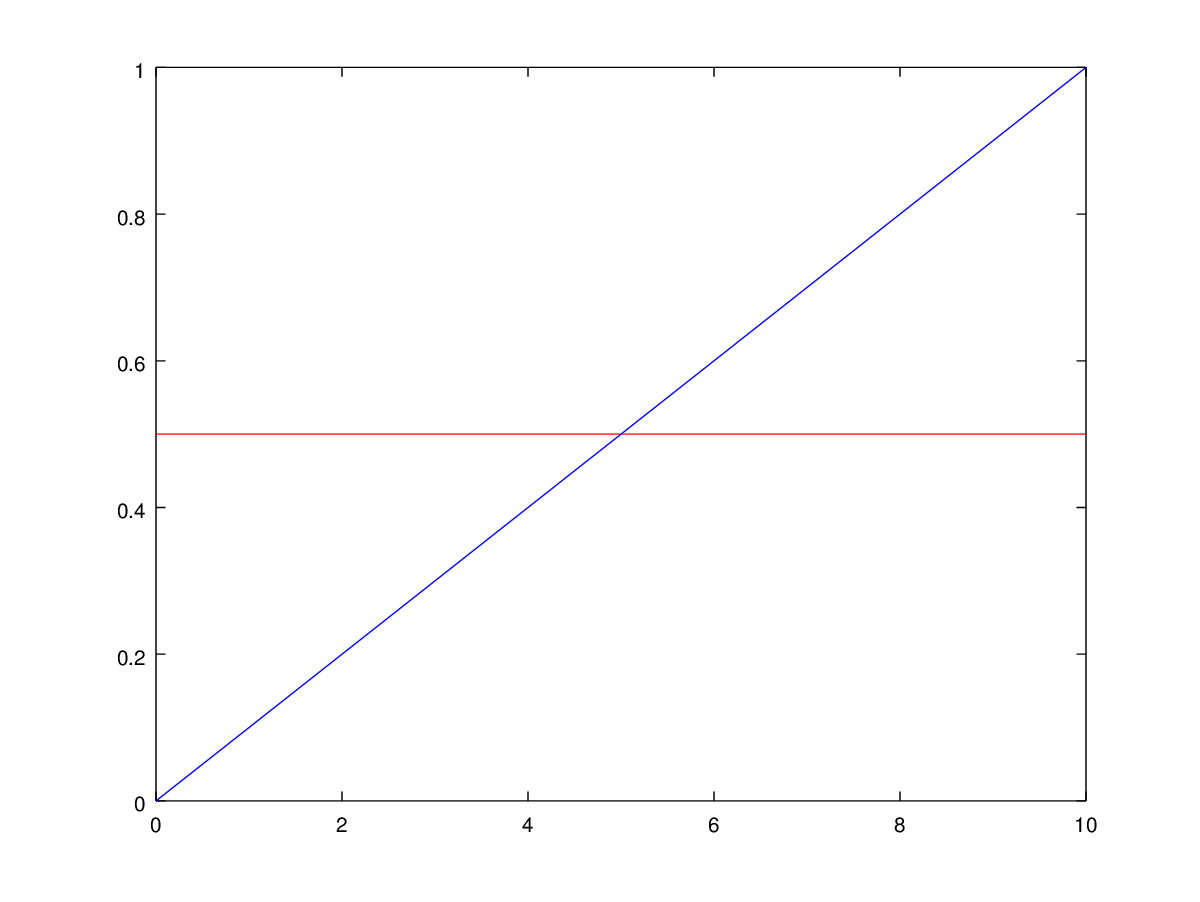
\includegraphics{expectation.png}
\label{fig:expectation}
}
\end{figure}
Clearly, for swipe gesture navigation, it is reasonable to assume that the time required increases proportionally with the distance as the number of swipes increases proportionally as well.
It is also reasonable to assume constant time consumption for menu navigation as the page selection process should be independent of $d$. However, this might not hold true when $d$ is so large that
the user is required to scroll within the menu in order to select the desired page. In Figure \ref{fig:expectation}, we presume the intercept point between the lines to exist. The location, however,
is part of our research.
The user satisfaction is likely to be a monotonically decreasing function in $d$. However, the shape of the function is unknown and will be subject to our research as well.

The results of our research will give important insight into the usability of different navigation methods, potentially leading to guidelines for the design of future e-learning apps.
\section{Related Work}

\section{Study Design}
\subsection{Conceptual Design}
\subsubsection{Tasks}
In order to simulate the scenarios of jumping from one question to another, we develop a series of treasure hunt like tasks. Here, the goal is to find the treasure which
is hidden behind a door. A door is represented by a page. Starting at the first page, an instruction displayed on the bottom of the screen guides the participant to the next one
by exactly telling them the number of the next door. When the participant has opened the respective door, the next
instruction is displayed. The distance to cover from one door to another is always in the same small range for each task. However, the distances differ for
different tasks. Consider the example in Figure \ref{fig:puzzle} which has distances in range two to three. The arrows indicate the door to open in
the next step. Hence, the sequence of doors to open in order to reach the treasure is 1, 3, 6, 4, 2, 5.
\begin{figure}
\caption{An example of a puzzle}
\resizebox{\columnwidth}{!}{
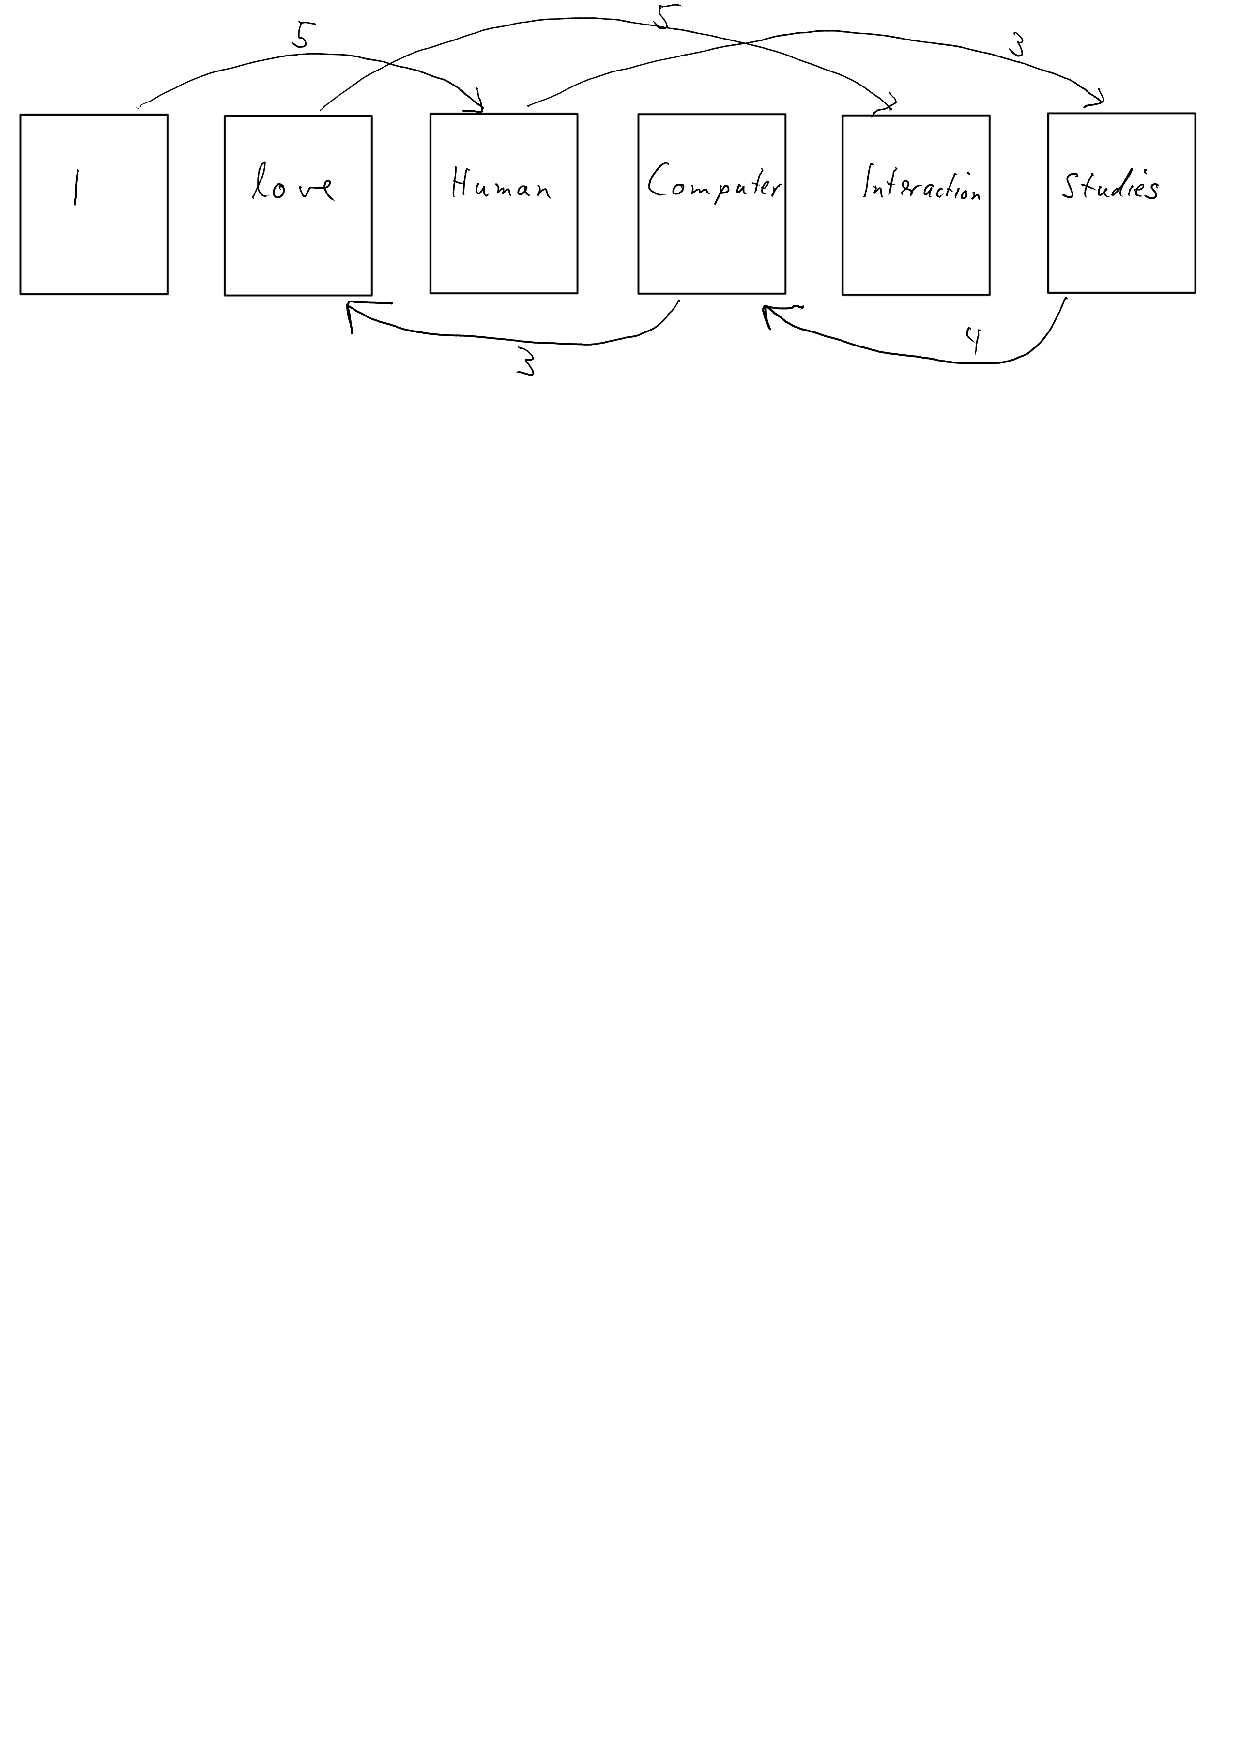
\includegraphics[clip, trim=0cm 23cm 0cm 0cm]{schnitzeljagd.pdf}
\label{fig:puzzle}
}
\end{figure}
The tasks cannot be failed to be completed. That is, there is no way to open the doors in the wrong order or to require too much time. This implies that we also do not measure effectiveness.

To avoid any bias of learning effects
the concrete permutation of tasks is generated by subsequently drawing
(uniformly at random, without returning) from the remaining tasks.

\subsubsection{Measures}
As stated above, we aim to measure the dependent variables efficiency and satisfaction of the two navigation methods. 
\paragraph{Efficiency} For the efficiency, we measure the time required to open the door which has to be opened next. We start measuring at the point
when the previous door was opened, that is, when the next instruction is displayed.
\paragraph{Satisfaction}
In order to assess the user satisfaction depending on the distance, after each task, the user is asked to rate their
satisfaction with the treasure hunt. We retrieve this information through a poll that is built into the application and pops
up after the last door is reached.
After completing the entire task set, the participant is asked to fill in the following questionnaire:
\begin{enumerate}
  \item Gender / Age
  \item Number of years of experience with smartphones
\end{enumerate}

\subsubsection{Randomized Split-Plot Design}
For our study, we decided for a between-group design for two reasons.
First, when solving the tasks with the second type, the test persons might rate their satisfaction more drastically, as they
are biased from having solved the tasks with the respective other navigation method.
Secondly, in order to avoid an extreme learning effect, the tasks for swipe gesture navigation and menu navigation
would have to be distinct if a within-group design were used. This should be avoided to ensure comparability.
The participants are assigned to each task randomly (at uniform) by
employing the random number generator of the respective android device.

\subsubsection{Participants}
As we thrive for an experiment duration of less than 15 minutes,
the participants can be acquisited in the field.
For the location we chose the dining hall of a local university,
since we can expect students to have basic knowledge about handling mobile devices.
After verifying this assumption, they can directly perform the task in-place.
Students are the target audience of the e-learning application,
for which this study is conducted.
We can thus assume that our sample is representative.
\subsection{Realization of the Experiment}
We developed a simple Android application:
\subsubsection{GUI}
put a qt mock-up here
\subsubsection{How we measured efficiency}
maybe we don't need this\ldots?
\section{Experiments and Results}
\section{Discussion}

\section{Conclusions}
Conclusions
%\end{document}  % This is where a 'short' article might terminate

%ACKNOWLEDGMENTS are optional
\section{Acknowledgments}

%
% The following two commands are all you need in the
% initial runs of your .tex file to
% produce the bibliography for the citations in your paper.
\bibliographystyle{abbrv}
\bibliography{hci}  % sigproc.bib is the name of the Bibliography in this case
% You must have a proper ".bib" file
%  and remember to run:
% latex bibtex latex latex
% to resolve all references
%
% ACM needs 'a single self-contained file'!
%
%APPENDICES are optional
%\balancecolumns
\appendix
%Appendix A
\section{Some Appendices}
\end{document}
